\section{Strongly-Coupled Dark Matter}\label{sec:darkqcd}

\begin{figure}[htb!]
\centering
\twofigeqh{figures/comp_limit_dijet_new_svj_monojet_2d.pdf}{{figures/comp_gq_dijet_orig_svj_monojet_rinv0.3}.pdf}
\caption{Excluded regions of the \mZprime-\rinv plane (left) and limits on \gq (right) from the SVJ search, dijet search, and monojet search.
}
\label{fig:svjexcl}
\end{figure}

\begin{figure}[htb!]
\centering
\twofigeqh{figures/axol1tl_score_schan.pdf}{figures/axol1tl_score_tchan2.pdf}
\caption{Score distributions from anomaly triggers on SVJ processes. (PLACEHOLDER)}
\label{fig:svjanomaly}
\end{figure}

\begin{figure}[htb!]
\centering
\twofigeqh{figures/rocScoreSigP2DQCD_rinv.pdf}{figures/WNAE_performance_from_SVJ_t_channel_status_update_2024_02_06-2.pdf}
\caption{The performance of the latest SVJ taggers: supervised ParticleNet (left) and unsupervised Wasserstein normalized autoencoder (right).
A score of 1.0 would indicate perfect discrimination between signal and background jets.}
\label{fig:svjtaggers}
\end{figure}

% centered, fixed-width column type
\newcolumntype{C}[1]{w{c}{#1}}
\newlength\searchlen
\setlength\searchlen{1cm}
\newlength\searchlena
\setlength\searchlena{2\searchlen}
\newlength\searchlenb
\setlength\searchlenb{3\searchlen}
\newlength\searchlenc
\setlength\searchlenc{6\searchlen}

\begin{table}[!hbtp]
\vspace{\myfigurespacing}
\centering
\begin{tabular}{c|*{6}{C{\searchlen}}}
\hline
\multirow{2}{*}{Mediator} & \multicolumn{6}{C{\searchlenc}}{Mass range} \\
& \multicolumn{2}{C{\searchlena}}{Low} & \multicolumn{2}{C{\searchlena}}{Medium} & \multicolumn{2}{C{\searchlena}}{High} \\
\hline
\PZprime & \multicolumn{2}{C{\searchlena}}{\cellcolor{yellow!50}\makecell{standard\\(boosted)}} & \multicolumn{2}{C{\searchlena}}{\cellcolor{magenta!50}\makecell{scouting\\\vphantom{(boosted)}}} & \multicolumn{2}{C{\searchlena}}{\cellcolor{orange!50}\makecell{standard\\\vphantom{(boosted)}}} \\
\hline
\Pbifun & \multicolumn{3}{C{\searchlenb}}{\cellcolor{orange!50}\makecell{standard\\\vphantom{(boosted)}}} & \multicolumn{3}{C{\searchlenb}}{\cellcolor{magenta!50}\makecell{scouting\\\vphantom{(boosted)}}} \\
\hline
\end{tabular}
\vspace{\myfigureskip}
\caption{A summary of the conventional trigger options to target different mediators and mass ranges for SVJ production.}
\label{tab:conventional}
\end{table}

% todo: add plot showing discovery significance for Run 2 vs Run 3, taking into account sqrt(s), lumi

\begin{figure}[htb!]
\centering
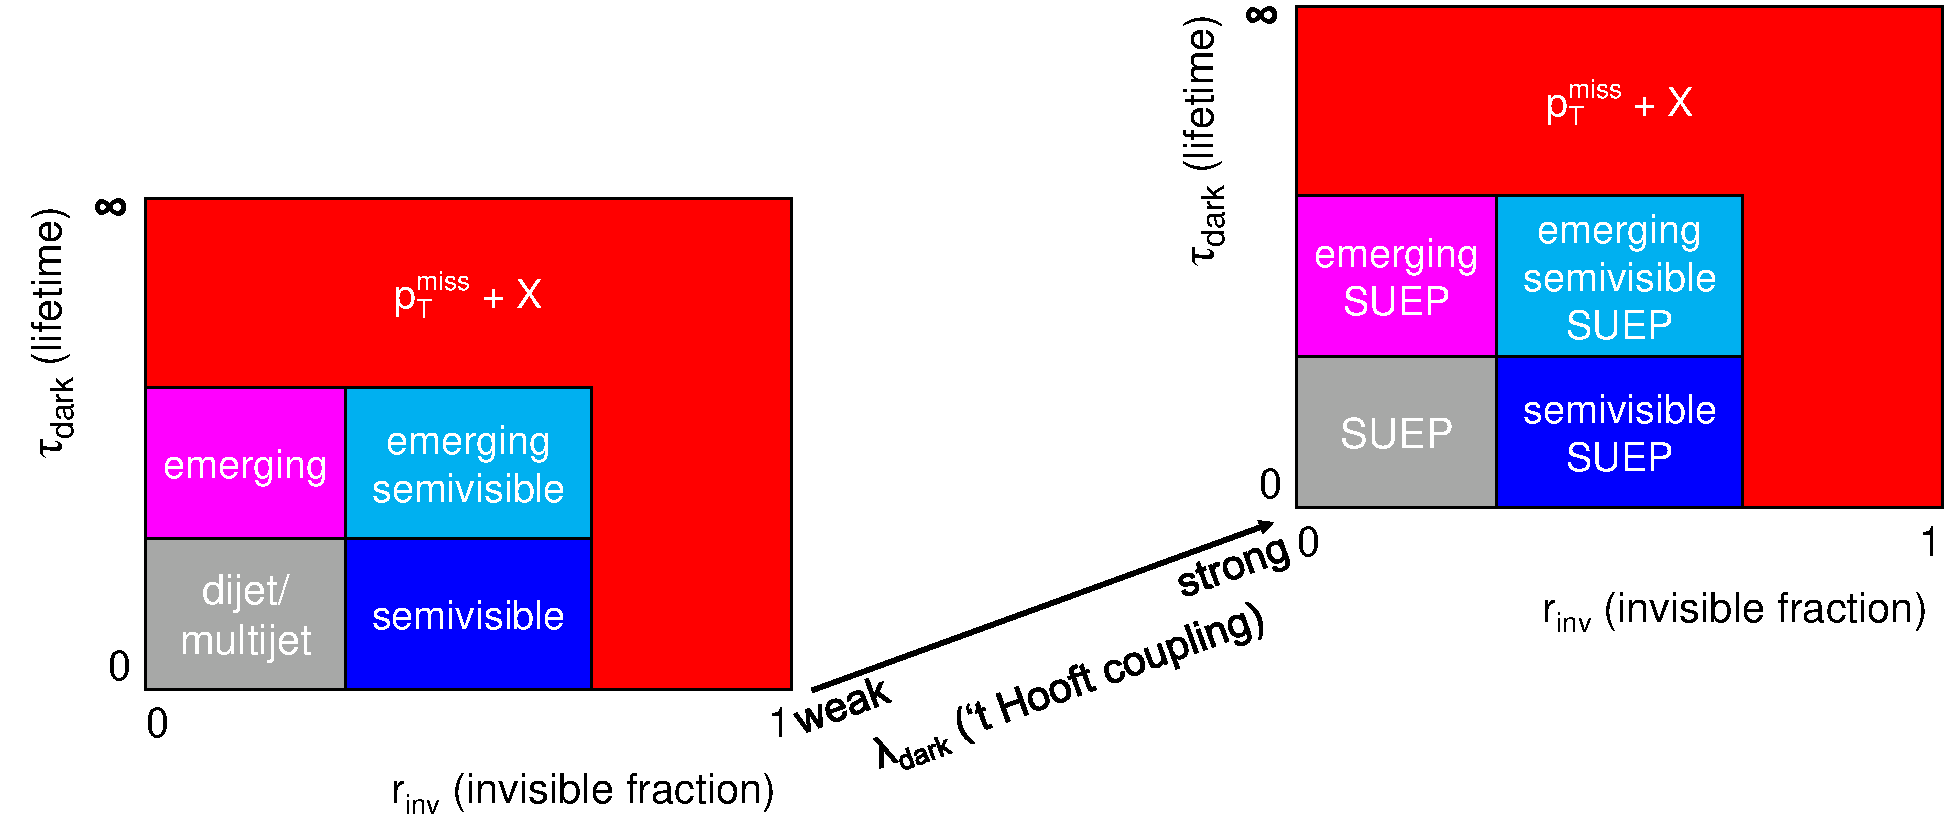
\includegraphics[width=0.95\myfigurewidth]{figures/svj_acceptance_diagram_v7.pdf}
\caption{A diagram illustrating the phenomena and search strategies with maximal acceptance for different combinations of dark QCD parameters.}
\label{fig:svjacc}
\end{figure}
